%%%%%%%%%%%%%%%%%%%%%%%%%%%%%%%%%%%%%%%%%%%%%%%%%%%%%%%%%%%%%%%%%
% Tese de Doutorado / Dept. Fisica, CFM, UFSC                   %
% Lacerda@CórregoGrande - Jan/2018                              %
%%%%%%%%%%%%%%%%%%%%%%%%%%%%%%%%%%%%%%%%%%%%%%%%%%%%%%%%%%%%%%%%%

%:::::::::::::::::::::::::::::::::::::::::::::::::::::::::::::::%
%                                                               %
%                           Anexo DR2                           %
%                                                               %
%:::::::::::::::::::::::::::::::::::::::::::::::::::::::::::::::%

\chapter{Participação no segundo {\em data-release} do CALIFA}
\label{apendice:DR2}

A confiança na qualidade dos dados observacionais é primordial para o desenvolvimento de qualquer estudo empírico. Sempre que um conjunto de dados tão grande passa por um processo complexo, como a síntese de populações estelares, a análise espectro por espectro se torna impossível, necessitando um arcabouço de programas que checam a qualidade da síntese. Esse procedimento, em muitos casos, acaba também funcionando como sensor da qualidade dos espectros observados. O processo ficou descrito e publicado no artigo do DR1 e foi repetido nos conseguintes. No primeiro {\em data-release} do CALIFA nosso grupo de populações estelares se encarregou dessa tarefa, utilizando a síntese com o \starlight. No segundo eu escrevi os programas da análise da qual as discussões, e três figuras, entremeiam o artigo da colaboração\citep{GarciaBenito.etal.2015a}. Para o último {\em data-release}, a análise publicada foi feita através de outro grupo dentro do projeto CALIFA. Mesmo assim, seguindo a linha dos dois primeiros, a repeti utilizando os resultados do \starlight como controle de qualidade dos nossos ajustes espectrais. Comparações com os resultados das amostras anteriores mostram uma importante e gradativa melhora nos espectros residuais.

%---------------------------- Figure ----------------------------
\begin{figure}
	\centering
	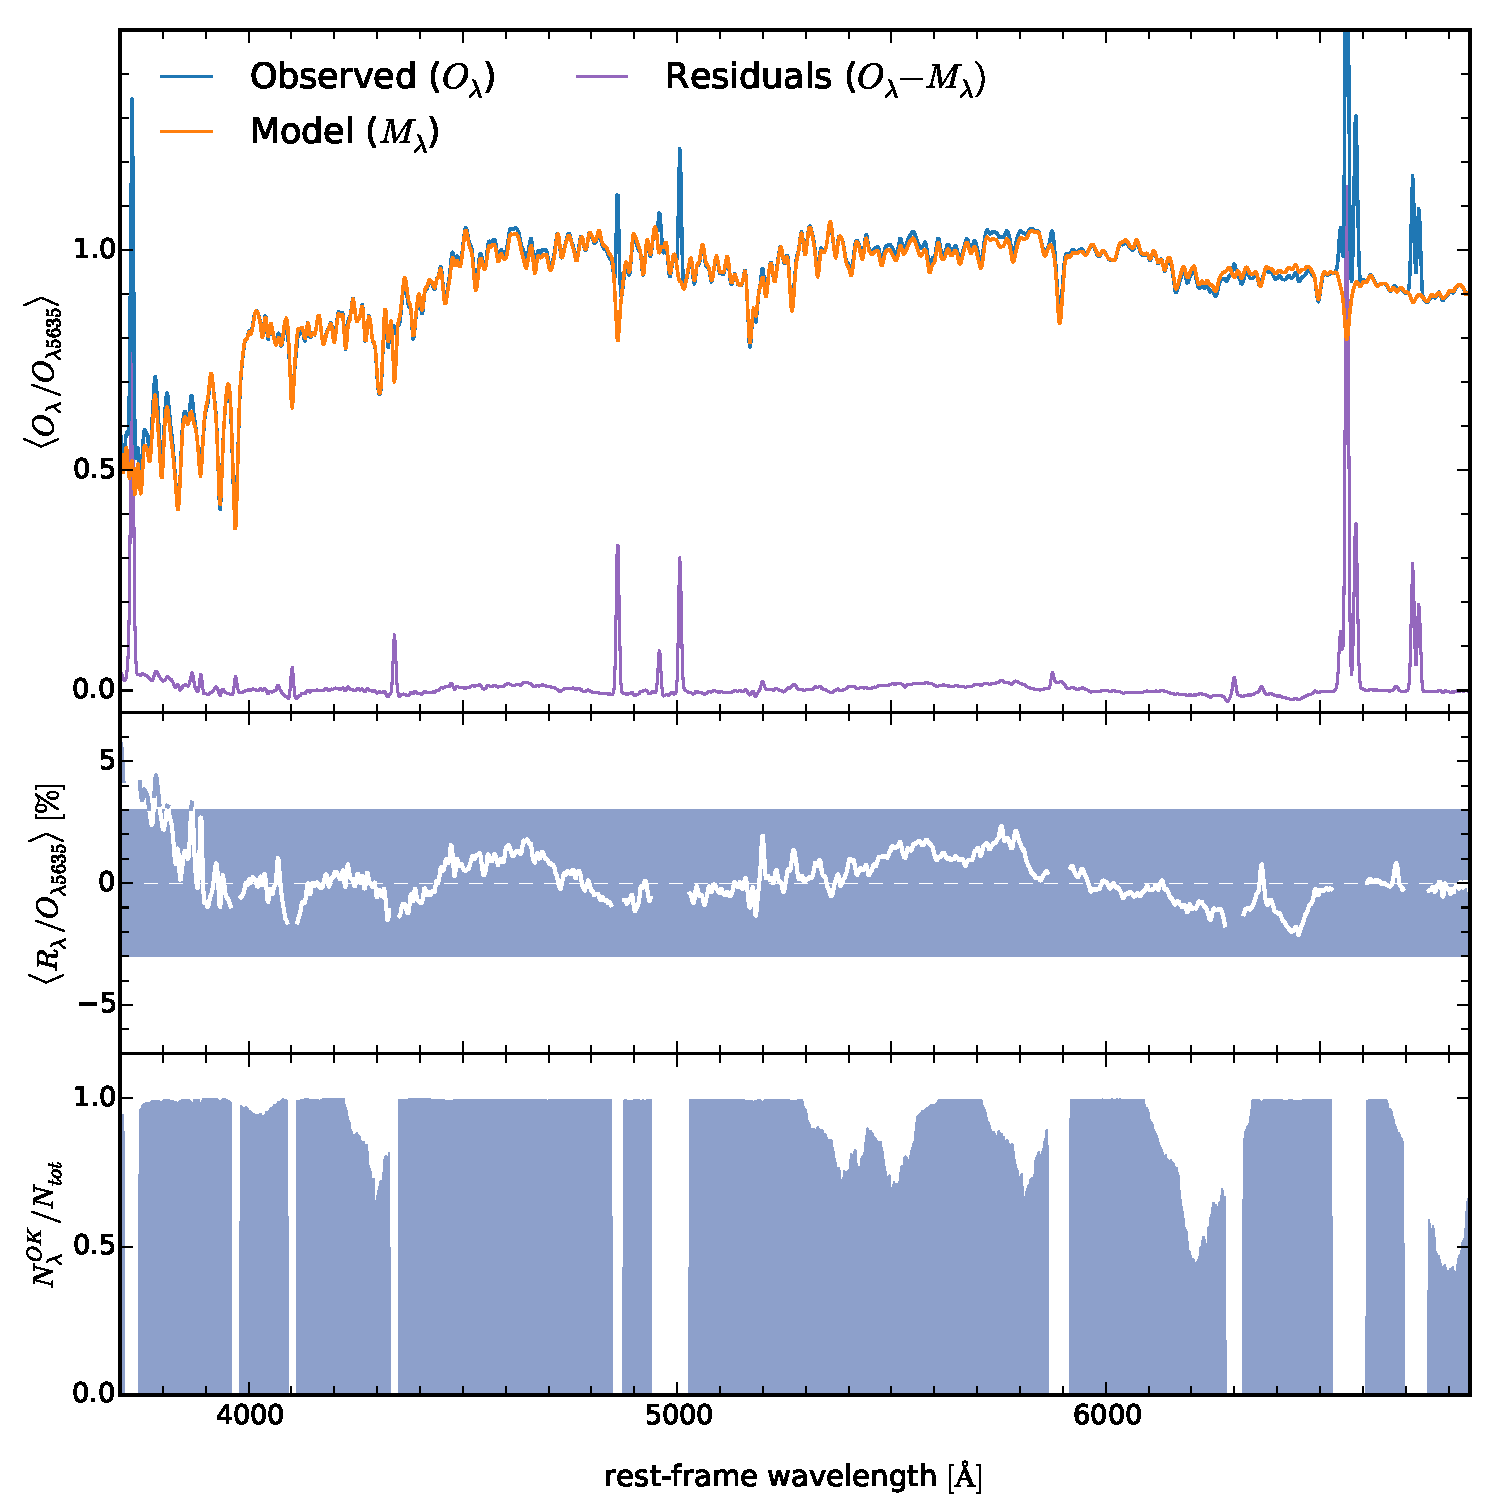
\includegraphics[scale=0.6]{figuras/DR2_spectral_residuals.pdf}
	\caption[DR2: Espectros médios: observado, sintético e residual]
	{{\ATR \ojo falta caption!!}
	Retirado de \citet{GarciaBenito.etal.2015a}.}
  \label{fig:obs_syn_res}
\end{figure}
%---------------------------- Figure ----------------------------

O espectro observado médio de $170\,670$ zonas presentes no DR2 aparece no primeiro painel da Figura \ref{fig:obs_syn_res}. Antes, cada espectro de cada zona é normalizado pelo fluxo da janela de 90 \AA\ ao redor de 5635 \AA. Na mesma figura temos os espectros sintético médio (linha laranja) e residual médio (linha roxa). No painel central vemos um {\em zoom} do espectro residual e, em destaque pintado de azul, o intervalo entre $\pm 3$\%. Nele as linhas de emissão e píxeis defeituosos mascarados durante o processo da síntese estão removidos. Finalmente, no último painel, a fração de píxeis não mascarados para cada $\lambda$. Essa figura deve ser comparada com a Figura 13 do artigo \citet{CidFernandes.etal.2014a}, mostrando que a nova versão do pacote de redução dos dados leva a menores resíduos, principalmente na parte azul do espectro ($\lambda <$ 5000 \AA).

{\ATR
\ojo em algum lugar tem que explicar a logica desses testes: Eles assumem que o modelo tah certo e que os residuos sao devido a problemas com os dados, tanto ruido como problemas sistematicos com a calibracao...

\ojo alem disso me pergunto se na vale apena colar a fig 13 de CF+14
}

%---------------------------- Figure ----------------------------
\begin{figure}
	\centering
	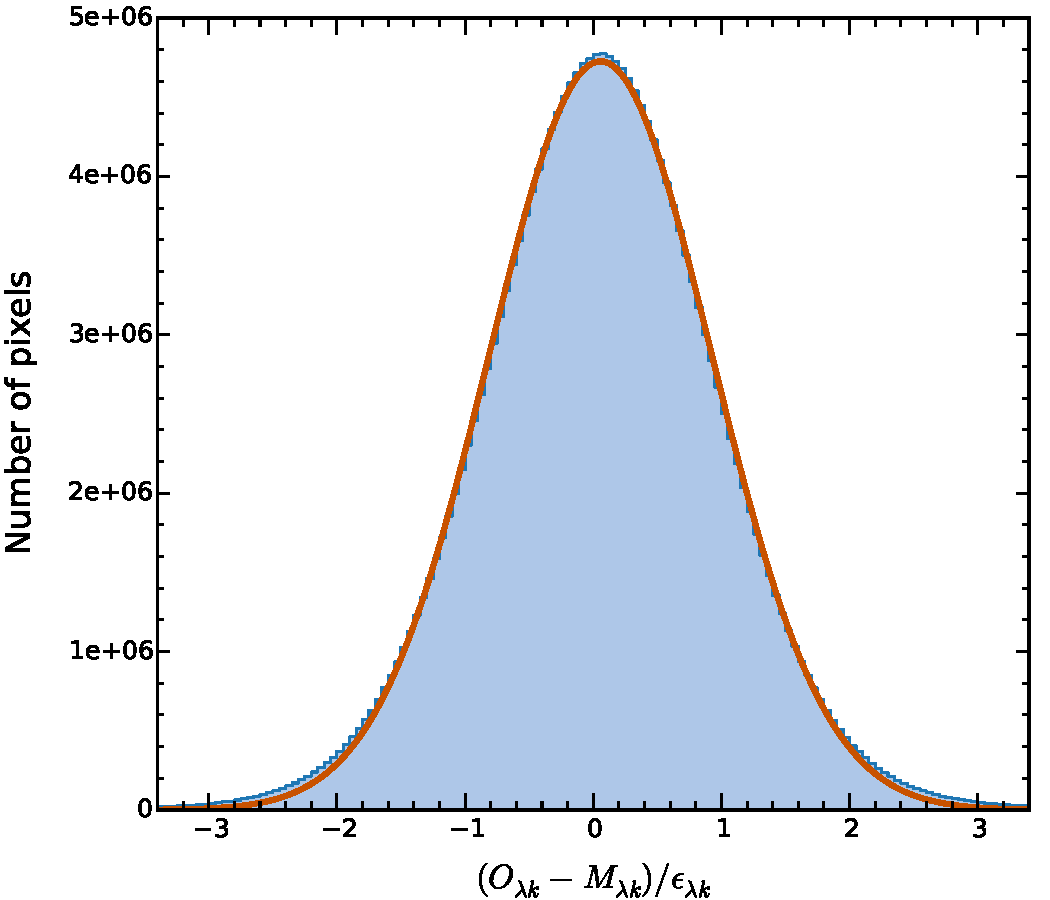
\includegraphics[scale=0.4]{figuras/DR2_hist_error.pdf}
	\caption[DR2: Distribuição dos resíduos reduzidos]
	{Distribuição do resíduo reduzido, $(O_{\lambda,k} - M_{\lambda,k})/\epsilon_{\lambda,k}$, para todos os comprimentos de onda $\lambda$ e todos os espectros $k$ de todas as galáxias presentes no DR2 ($209\,151\,086$ pontos no total). A linha laranja mostra o melhor ajuste Gaussiano para a distribuição (média $= 0.03$; $\sigma = 0.87$). Retirado de \citet{GarciaBenito.etal.2015a}.}
	\label{fig:fres_norm_error_distrib}
\end{figure}
%---------------------------- Figure ----------------------------

A Figura \ref{fig:fres_norm_error_distrib} põe à prova a qualidade dos ajuste espectrais e também dos erros formais estimados para cada comprimento de onda. Supondo que um espectro residual seja inteiramente formado por ruído, ou seja, modelos estelares e ajustes tão bons quanto se possam ter, sua distribuição deveria ser gaussiana e centrada em zero. Além disso, quando temos um erro formal no fluxo perfeitamente estimado, a distribuição do espectro residual normalizado pelo erro formal no fluxo deveria ser formada basicamente de ruído, por isso, centrada em zero e com $\sigma \sim 1$. Nessa figura vemos o histograma do resíduo reduzido, ou seja, a diferença entre o fluxo observado ($O_{\lambda,k}$) e o modelado ($M_{\lambda,k}$), obtido através da síntese com o \starlight, dividida pelo erro associado ($\epsilon_{\lambda,k}$). Os índices $\lambda$ e $k$ representam um certo comprimento de onda de um certo espectro respectivamente. Dessa análise são excluídos intervalos em $\lambda$ que representam linhas de emissão e dados espúrios. A distribuição é muito bem descrita por uma gaussiana com centro 0.03 e $\sigma = 0.87$, ambos muito próximos dos valores óptimos.

\begin{figure}
	\centering
	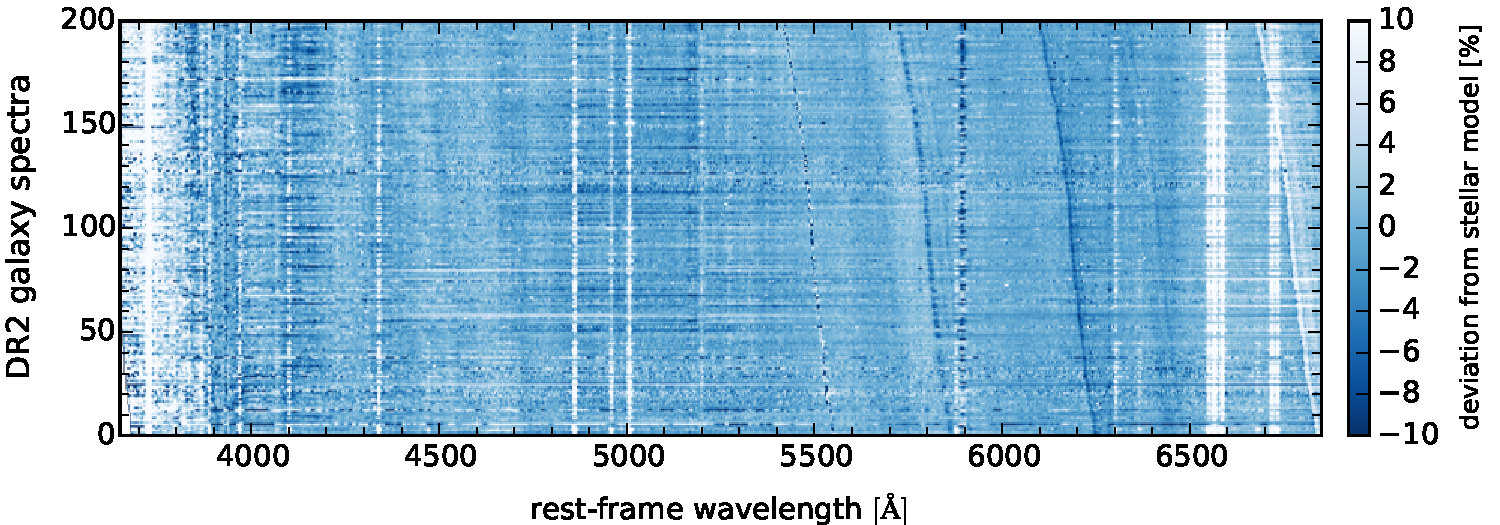
\includegraphics[scale=0.5]{figuras/DR2_stacked_residuals.pdf}
	\caption[DR2: Espectros residuais nucleares]
	{Desvio relativo entre o espectro observado e o modelado pela síntese, ($O_\lambda - M_\lambda$)/$O_\lambda$, Para as regiões nucleares de todas as galáxias presentes no DR2, ordenadas por redshift. As linhas verticais nos mostram desvios sistemáticos do modelo e, as inclinadas, modelos imperfeitos do céu, como remoção de linhas telúricas. Retirado de \citet{GarciaBenito.etal.2015a}.}
	\label{fig:fnuc_stack}
\end{figure}

A Figura \ref{fig:fnuc_stack} é formada pelos espectros nucleares, ajustados para o referencial de laboratório, das 200 galáxias presentes no DR2 e ordenados por {\em redshift}. As cores codificam o desvio relativo entre o fluxo observado e o modelado $(O_\lambda - M_\lambda)/O_\lambda$, sem nenhuma máscara espectral. As linhas verticais mostram os desvios sistemáticos dos modelos do \starlight, presentes no refericial de laboratório (e.g., modelos estelares imperfeitos, linhas de emissão). Já as linhas inclinadas mostram desajustes no referencial de observação (e.g., modelo imperfeito do céu). Esta análise nos ajudou a melhorar a máscara de remoção de linhas telúricas e linhas de emissão dos espectros.


% End of this chapter
